\documentclass{../../slides-style}

\slidetitle{Практика по архитектуре}{25.04.2025}

\begin{document}

    \begin{frame}[plain]
        \titlepage
    \end{frame}

    \begin{frame}{Реверси}
        \begin{columns}
            \begin{column}{0.7\textwidth}
                \begin{itemize}
                    \item Поле 8 на 8, чёрные и белые фишки
                    \item Игроки по очереди делают ходы
                    \item Каждая выставленная на доску фишка меняет цвет всех фишек между собой и фишкой такого же цвета
                    \item Побеждает тот, фишек чьего цвета в конце больше
                \end{itemize}
            \end{column}
            \begin{column}{0.3\textwidth}
                \begin{center}
                    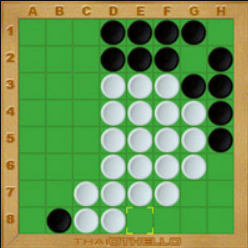
\includegraphics[width=0.8\textwidth]{reversi.png}

                    \vspace{1cm}

                    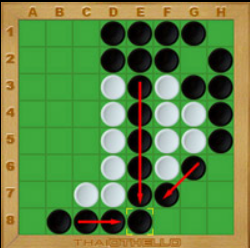
\includegraphics[width=0.8\textwidth]{reversi2.png}
                \end{center}
            \end{column}
        \end{columns}
        \attribution{\url{https://ru.wikipedia.org/wiki/Реверси}}
    \end{frame}

    \begin{frame}{Задача}
        \begin{itemize}
            \item Поделиться на команды по 2-3 человека
            \item Создать проект на \url{https://www.drawio.com/} или в любом другом UML-редакторе
            \item Спроектировать игру в реверси с пользовательским интерфейсом
            \begin{itemize}
                \item Должно быть можно играть двум людям против друг друга или человеку против бота одного из трёх уровней сложности
                \item Диаграмма должна быть довольно подробным проектом системы
            \end{itemize}
        \end{itemize}
    \end{frame}

\end{document}
